\documentclass[a4paper, 10pt, conference]{ieeeconf}      

% This command is only needed if you want to use the \thanks command
\IEEEoverridecommandlockouts                              
\overrideIEEEmargins
% See the \addtolength command later in the file to balance the column lengths
% on the last page of the document


%\usepackage{graphics} % for pdf, bitmapped graphics files
%\usepackage{epsfig} % for postscript graphics files
%\usepackage{mathptmx} % assumes new font selection scheme installed
%\usepackage{times} % assumes new font selection scheme installed
%\usepackage{amsmath} % assumes amsmath package installed
%\usepackage{amssymb}  % assumes amsmath package installed
\usepackage{graphicx}% http://ctan.org/pkg/graphicx
\usepackage{comment}

\title{\LARGE \textbf{Capita selecta: AI Topics} \\ 
Automatic Statistician}


\author{Rick van Hek, Mathias Van Herreweghe}


\usepackage[T1]{fontenc}
\usepackage{graphicx}
\usepackage{lipsum}
\usepackage{verbatim}
\usepackage{amsbsy}
\usepackage{amsmath}
\usepackage{amsfonts}
%\usepackage{flushend}
\usepackage[colorinlistoftodos]{todonotes}
\let\proof\relax
\let\endproof\relax
\usepackage{amsthm}
\newtheorem{theorem}{Theorem}

\pagenumbering{arabic}

\begin{document}

\maketitle
\thispagestyle{plain}
\pagestyle{plain}


\tableofcontents

\section{Introduction}
Interpreting and predicting data is not convenient without some sort of visual representation, let alone making assumptions or discovering insights about it. Due to the fact that making a model that can visualize the data is rather time intensive, people have devoted time to automate this. This is not restricted to only making a more visually appealing model, but also generating natural language descriptions about the model. In this paper we will mainly be describing the early system: \textit{Automatic Bayesian Covariance Discovery (ABCD)}~\cite{lloyd2014automatic}. This system describes an open-ended language of Gaussian process models through a compositional grammar. Because of the compositional structure of the grammar, the system allows a way to generate natural-language descriptions of the structure.\\
The capabilities will be tested in a comparison versus our own manually achieved predictions and data interpretations on a regression and a time series dataset.


\section{The Automatic Statistician}
The Automatic Statistician (AS) will model a given dataset by using \textit{Gaussian Processes} which in turn use \textit{Kernels}. It does this in an iterative way, improving the kernels each iteration in order to get the best fitting model. Once a good model is found, it will then create an extensive report in natural language.
\subsection{Gaussian process}
A Gaussian process will model a distribution over multiple functions. Think of it as this way; if you have data, and you want to automatically find a function describing this data, you don't really know how many parameters you need. You want a way of not having to specify how many parameters the function should have. For example if you have a set of data points, you can model them by a very `spikey' function, such as in figure~\ref{fig:examplediagram}. But a better model would be a smoother function such as in figure~\ref{fig:examplediagram_vloeiend}. But this would require a lot more parameters.

\begin{figure}[!ht]
    \centering
    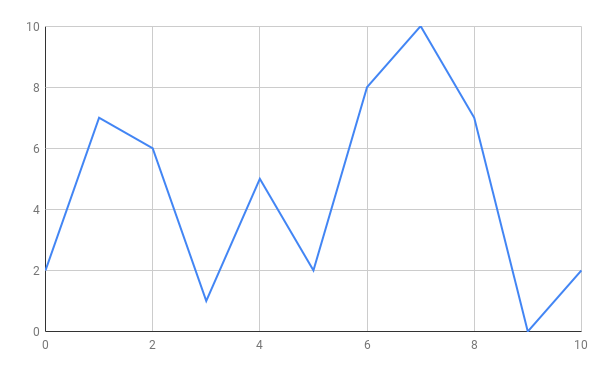
\includegraphics[width=0.6\linewidth]{report/images/examplediagram.png}
    \caption{}
    \label{fig:examplediagram}
\end{figure}
\begin{figure}[!ht]
    \centering
    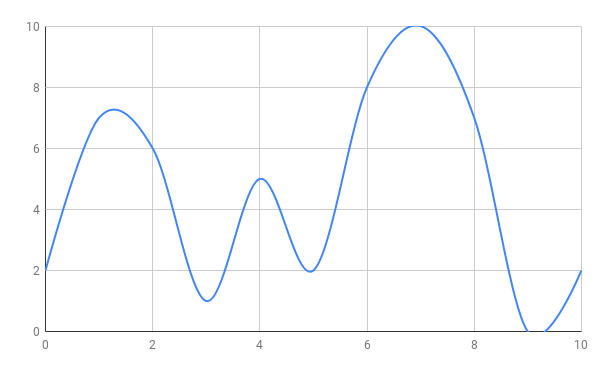
\includegraphics[width=0.6\linewidth]{report/images/examplediagram_vloeiend.png}
    \caption{}
    \label{fig:examplediagram_vloeiend}
\end{figure}

That's why Gaussian processes (GP's) are non-parametric, and have only two inputs: a mean function (\ref{eq:meanfunction}) and kernel (or covariance) function (\ref{eq:kernelfunction}). This mean- and kernel function will ensure this `smoothness'.

\begin{equation}\label{eq:meanfunction}
    \mu (x) = \mathbb{E}(f(x))
\end{equation}


\begin{equation}\label{eq:kernelfunction}
    k(x,x') = Cov(f(x), f(x'))
\end{equation}

The kernel function depicts a sort of similarity measure. If x and x', which are two input values, are close to each other, we expect the output to be close to each other as well. This will make sure the output is not too `spikey'.

So when a Gaussian Process is given (with a kernel and mean function), one can calculate the marginal likelihood of given data. You can also get a predictive distribution for new points, if you have already have existing data.

\subsection{The kernels}
\label{subsec:as:kernels}
This open-ended language (ABCD) has multiple kernels in it's grammar, each describing a certain `feature' of a possible function. ABCD supports five different kernels that each encode something else:
\begin{itemize}
    \item White Noise (WN): uncorrelated noise
    \item Constant (C): constant functions
    \item Linear (LIN): linear functions
    \item Squared Exponential (SE): smooth functions
    \item Periodic (PER): periodic functions
\end{itemize}

ABCD further supports two compositional rules, that allows to combine kernels and make more complex kernels. There is a rule to add (\ref{eq:compositionalrule_addition}) and multiply (\ref{eq:compositionalrule_multiply}) kernels.

\begin{equation}
    \label{eq:compositionalrule_addition}
    (k_1 + k_2)(x, x_0) = k_1(x, x_0) + k_2(x, x_0)
\end{equation}

\begin{equation}
    \label{eq:compositionalrule_multiply}
    (k_1 \times k_2)(x, x_0) = k_1(x, x_0) \times k_2(x, x_0)
\end{equation}

For example one could combine the Squared Exponential ($SE$) kernel with the Periodic ($PER$) kernel by multiplying these ($SE \times PER$), which will yield a kernel to approximate periodicity in the model.

Another operator has been added to the grammar, allowing change points to be incorporated. This is essential especially in Time Series data. Because the behavior of data could suddenly drastically change, such as in figures~\ref{fig:changepointexample} and~\ref{fig:changewindowexample}.
Changepoints are defined through addition and multiplication with sigmoidal functions:


\begin{equation}
    \label{eq:changepoint_1}
    \boldsymbol{CP}(k_1, k_2) = k_1 \times \boldsymbol{\sigma} + k_2 \times \boldsymbol{\bar{\sigma}}
\end{equation}

Where $\boldsymbol{\sigma} = \sigma(x)\sigma(x')$ and $\boldsymbol{\bar{\sigma}} = (1 - \sigma(x))(1 - \sigma(x'))$.

What this essentially does is split a function domain into two sides, and applies the corresponding kernel functions on their respective side. As seen in figure~\ref{fig:changepointexample}, the data suddenly changes in 1975. This changepoint will split up the data, and apply the two different kernels to both sides. These kernels could still change in further iterations of the searching process.

\begin{figure}[ht!]
    \centering
    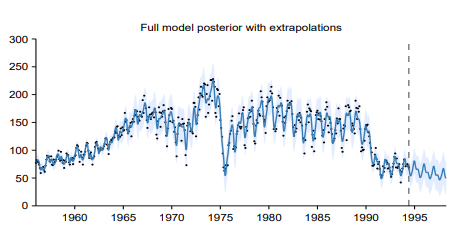
\includegraphics[width=\linewidth]{report/images/timeserieschangepoint.png}
    \caption{Example of a change point for time series data in the year 1975.~\cite{theautomaticstatistician:sulphuric}}
    \label{fig:changepointexample}
\end{figure}

The final operation that has been added is the Change-Window (CW) operation, which basically applies the CP operation twice, on two different change points. In figure~\ref{fig:changewindowexample} this can be seen from year 1650 until 1710. It will apply a different kernel within that time frame.

\begin{figure}[ht!]
    \centering
    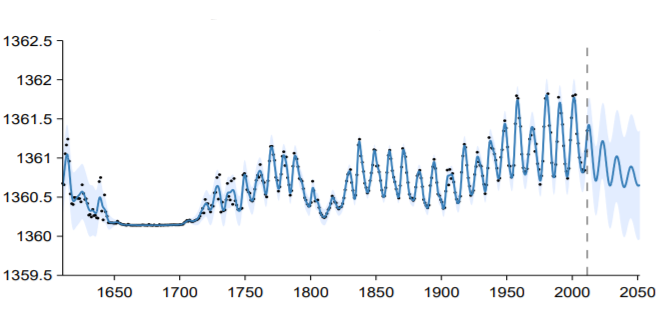
\includegraphics[width=\linewidth]{report/images/timeserieschangewindow.png}
    \caption{Example of a change window for time series data from the year 1650 until 1710.~\cite{theautomaticstatistician:solar}}
    \label{fig:changewindowexample}
\end{figure}


The base kernels have been expanded and reparameterised to allow for easier automatic translation to natural language description. These can be seen in table~\ref{tab:regressionmodelkernel}.

\begin{table}[!ht]
\begin{tabular}{ll}
Regression model                                & Kernel                    \\ \hline
\multicolumn{1}{l|}{GP smoothing}               & $SE + WN$                 \\
\multicolumn{1}{l|}{Linear regression}          & $C + LIN + WN$            \\
\multicolumn{1}{l|}{Multiple kernel}            & $\sum SE + WN$            \\
\multicolumn{1}{l|}{Trend, cyclical, irregular} & $\sum SE + \sum PER + WN$ \\
\multicolumn{1}{l|}{Fourier decomposition}      & $C + \sum cos + WN$       \\
\multicolumn{1}{l|}{Sparse spectrum GPs}        & $\sum cos + WN$           \\
\multicolumn{1}{l|}{Spectral mixture}           & $\sum SE \times cos + WN$ \\
\multicolumn{1}{l|}{Changepoints}               & e.g. $CP(SE, SE) + WN$    \\
\multicolumn{1}{l|}{Heteroscedasticity}         & e.g. $SE + LIN \times WN$
\end{tabular}
\caption{Common regression models expressible in their language. \textit{cos} is a special case of the reparametrised \textit{PER}~\cite{lloyd2014automatic}}
\label{tab:regressionmodelkernel}
\end{table}

\subsection{Searching for a model and evaluate}
ABCD uses \textit{Greedy Search} to compute the `best' model, which can be summarized by the following steps:
\begin{enumerate}
    \item it starts from the WN kernel (see subsection~\ref{subsec:as:kernels}),
    \item expanding the kernel expression using the grammar rules (defined below),
    \item optimizing the hyperparameters of these new (or expanded) kernels,
    \item evaluating this new set of kernels on the data,
    \item select the kernel with the best evaluation.
\end{enumerate}
Step 2 uses the grammar as defined below to expand the previously best kernel. Obviously in the beginning it is the WN kernel, but after each iteration it would have the previously best kernel as input. 

\begin{table}[!ht]
    \centering
    \begin{tabular}{ll}
        $\mathcal{S} \rightarrow \mathcal{S} + \mathcal{B}$   & $\mathcal{S} \rightarrow \mathcal{S} \times \mathcal{B}$ \\
        $\mathcal{S} \rightarrow CP(\mathcal{S},\mathcal{S})$ & $\mathcal{S} \rightarrow CW(\mathcal{S}, \mathcal{S})$   \\
        $\mathcal{S} \rightarrow \mathcal{B}$       & $\mathcal{S} \rightarrow C$         
    \end{tabular}
\end{table}

$\mathcal{S}$ represents any kernel Subexpression, $\mathcal{B}$ represents a Base kernel, whereas CP, CW and C were previously defined in subsection~\ref{subsec:as:kernels}.\\
Step 3 uses the \textit{conjugate gradient method} to optimize the hyperparameters of the kernels. Step 4 will use \textit{Bayesian Information Criterion} (BIC) \cite{schwarz1978estimating} to give a BIC-score to all the kernels, and the kernel with the lowest score gets picked as the best one. The BIC of model $\mathcal{M}$ where $|\mathcal{M}|$ is the number of free parameters and data $\mathcal{D}$ where $|\mathcal{D}|$ is the number of data points is:
\begin{equation}
    \label{eq:bic}
    \textbf{BIC}(\mathcal{M}) = -2 \log p(\mathcal{D}|\mathcal{M}) + |\mathcal{M}| \log |\mathcal{D}|
\end{equation}
where $p(\mathcal{D}|\mathcal{M})$ can be seen as the marginal likelihood of the data $\mathcal{D}$.\\

These 5 steps will continue to iterate while there are still improvements on the previous iteration (so the new kernels evaluate to a better BIC score), or a certain search-depth has been reached. Noteworthy is that this could lead to a suboptimal solution. But that's not the focus of the Automatic Statistician, their focus is on making a model and associating a comprehensible report for humans to interpret.

\subsection{Automatic natural language description generation}
The last part of the Automatic Statistician is automatically generating a report in natural language showing the models, assumptions made, insights about the data and predictions. This report should be detailed, but in a way that non-experts would still be able to read it without too much problems. Since the main focus of our project is on making a fitting model and interpreting them, we won't go into much detail on how these models get converted into natural language. A more technical explanation can be found in the referenced papers, to which the reader is invited to read.\\

After finding the kernel with the best score, it is used to generate a natural-language description. This is done by converting the kernel to a canonical form by flattening the nested sums and products into a sum of products, and then simplifying some kernels into base kernels with modified parameters. For example: $SE \times SE \rightarrow SE^{*}, C \times k \rightarrow k^*$ for any $k$, and $WN \times k \rightarrow WN^*$ for any $k \in \{C, SE, WN, Per\}$.\\
When these steps are applied, the kernel will be in the form of a sum of products, where each product will be of the form:

\begin{equation}
    k \times \prod_m Lin^{(m)} \times \prod_n \boldsymbol{\sigma} ^{(n)}
\end{equation}

where $\boldsymbol{\sigma}(x,x') = \sigma(x) \sigma(x')$ and $k \in \{ 1, WN, C, SE, \prod_j, Per^{(j)}, SE \times \prod_j Per^{(j)}\}$

In this form, the following steps will create a sentence describing each component:
\begin{enumerate}
    \item Pick \textit{one} kernel in the product to be the noun.
    \item Convert that kernel to a string using predefined sentences. Each kernel type has a fixed string bound to it, which can be seen in table~\ref{tab:kerneltostring}~\cite{lloyd2014automatic}.
    \item The other kernels become \textit{post-modifier} expressions which again have their own table to convert them to natural language, as seen in table~\ref{tab:postmodifiertostring}~\cite{lloyd2014automatic}.
    \item Further refinements (insights, extra information calculated from the data) which we won't go into detail, these can be seen in the papers~\cite{lloyd2014automatic},~\cite{lloyd2015representation}.
\end{enumerate}

\begin{table}[!ht]
    \centering
    \begin{tabular}{ll|ll}
        WN  & "uncorrelated noise" & SE                  & "smooth function" \\
        Per & "periodic function"  & Lin                 & "linear function" \\
        C   & "constant"           & $\prod_j Lin^{'j)}$ & "polynomial"     
    \end{tabular}
    \caption{\textit{Kernel} types to description.}
    \label{tab:kerneltostring}
\end{table}

\begin{table}[!ht]
    \centering
    \begin{tabular}{ll}
        SE                                  & "whose shape changes smoothly"                 \\
        Per                                 & "modulated by a periodic function"             \\
        Lin                                 & "with linearly varying amplitude"              \\
        $\prod_j Lin^{(j)}$                 & "with polynomially varying amplitude"          \\
        $\prod_j \boldsymbol{\sigma}^{(j)}$ & "which applies from / until [changepoint]"
    \end{tabular}
    \caption{\textit{Post-modifier} expression to description.}
    \label{tab:postmodifiertostring}
\end{table}

\section{Creative part}
The Automatic Statistician's website contains examples of demo runs of the software \cite{as_examples}. The examples are the reports generated by the Automatic Statistician. We will replicate a manual machine learning procedure for two of the examples and compare our results to those of the report. We will make such a comparison for the affairs dataset \cite{doi:10.1086/260646} in subsection \ref{subsec:reg_affairs} and the airline passengers dataset \cite{airpax_dataset} in subsection \ref{subsec:ts_airpas}.

\subsection{Regression: affairs}
The affairs dataset consists of multiple variables, these are the gender of a person, the amount of years married, whether or not a person has children, the degree of religiousness, the level of education, the kind of occupation (higher number means more prestigious) and the rating of a person's relationship. The target variable is the amount of extra-marital affairs the person had. The gender and children variable were excluded from the Automatic Statistician's input, as these were the non-numeric variables, so we did the same.\\

The Automatic Statistician performs a regression analysis by comparing three simple strategies for linear models using 5 fold cross validation on half of the data. The strategy with the lowest cross validated prediction error has then been used to train a model with the same half of data. The results of the regression can be found in table \ref{table:as_affairs}, the result is expressed as the root mean squared error (RMSE) of the cross validation.

\begin{table}[!ht]
\centering
\begin{tabular}{| l | l |}
  \hline
  Method & Cross validated RMSE \\
  \hline
  Full linear model & 3.22 \\
  BIC stepwise & 3.31 \\
  LASSO & 3.33 \\
  \hline
\end{tabular}
\caption{Results regression analysis Automatic Statistician}
\label{table:as_affairs}
\end{table}

Another part of the analysis is that it gives a summary of the relation between variables and the target variable. It finds that the output affairs

\begin{itemize}
    \item decreases linearly with input rating (correlation $-0.25$),
    \item decreases linearly with input religiousness (correlation $-0.22$),
    \item increases linearly with input years married (correlation $0.16$),
    \item decreases linearly with input age (correlation $0.10$),
    \item increases linearly with input occupation (correlation $0.12$),
    \item decreases linearly with input education (correlation $0.04$).
\end{itemize}

The report then concludes with a critical evaluation of its used model, which we will not further discuss in this report.\\

We then took it to ourselves to produce a model that would yield a better score than that of the Automatic Statistician. We started by exploring the data. We searched for outliers in the data using scatterplots and boxplots for all variables. We did not see the need to prune or correct anything within the data based on these plots. We created two new variables, these are \textit{marriageScore} which is the number of years married times the rating of the marriage, and \textit{experienceScore}, which is the age times the level of education times the kind of occupation. We then did a correlation analysis on the variables to find which were correlated the most to the output, these correlations can be found in table \ref{table:correlation_affairs}.

\begin{table}[!ht]
\centering
\begin{tabular}{| l | l |}
  \hline
  Variable & Correlation score \\
  \hline
  yearsmarried &      0.187 \\
  age &               0.095 \\
  experienceScore &   0.076 \\
  occupation &        0.050 \\
  marriageScore &     0.037 \\
  education &        -0.002 \\
  religiousness &    -0.145 \\
  rating &           -0.280 \\
  \hline
\end{tabular}
\caption{Results correlation analysis}
\label{table:correlation_affairs}
\end{table}

We then create additional variables based on the three most correlated variables. We include the square, cube and square root of variables \textit{yearsmarried}, \textit{age} and \textit{experienceScore}. Subsequently we create different models and compare the root mean squared error in the same manner the Automatic Statistician did. The results of the regression analysis can be found in table \ref{table:results_affairs}.

\begin{table}[!ht]
\centering
\begin{tabular}{| l | l | l |}
  \hline
  Method & RMSE & RMSE* \\
  \hline
  Gradient Boosting Method & 3.66 & 3.71 \\
  Random Forest & 3.21 & 3.15 \\
  LASSO & 3.12 & 3.13 \\
  ElasticNet & 3.17 & 3.15 \\
  Kernel Ridge & 3.16 & 3.20 \\
  Support Vector Regression & 3.44 & NA \\
  \hline
\end{tabular}
\caption{Results regression analysis, rounded to 2 decimals (* original variables only, as used by Automatic Statistician)}
\label{table:results_affairs}
\end{table}

As can be seen, some models score better than the model with the lowest RMSE of Automatic Statistician. Among our models, LASSO scored the best, even on the original data, which is a surprise given that Automatic Statistician also used this model and scored worse. This may be due to scaling of the data and the actual LASSO implementation. We have used the sklearn library \cite{scikit-learn} for all of our models. \\

Another part of Automatic Statistician's report that we wanted to try to replicate or even improve upon was explore the relationship between the variables and the output. We did this exploration by means of partial dependence plots. As can be seen in figure \ref{fig:pdp}, the relationships are not just linear. The Automatic Statistician limits itself to linear models, which is why it also finds linear relationships between the variables and the output. We used the gradient boosting regressor model from the sklearn library \cite{scikit-learn} to create the plots. We can see that for the variable \textit{age} that as a person gets older, the number of affairs decrease until around 37 years old, and then increases again. Another remarkable outcome is that when we plot \textit{yearsmarried} against \textit{age}, we see that for people older than 50 and whom are married between 2.5 and 11 years, the amount of affairs is the highest. This increased amount of affairs is not existent for people younger than 42 years old. This contradicts with the insights found by the AS, where they see that the amount of affairs increases with years married, and decreases with age. But we found that when you combine these two, the opposite is true.

\begin{figure}[!ht]
    \centering
    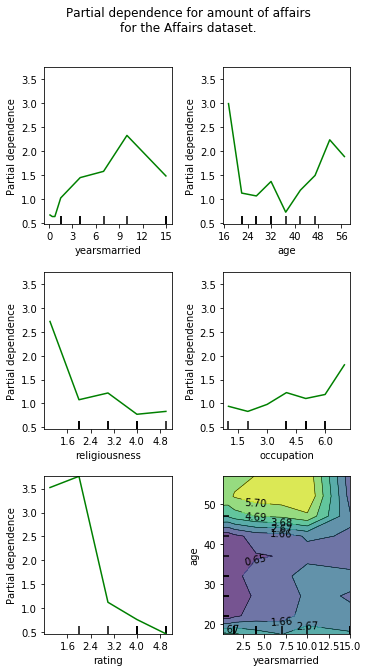
\includegraphics[width=\linewidth]{report/images/pdp.png}
    \caption{Partial dependence plots of multiple variables}
    \label{fig:pdp}
\end{figure}

\label{subsec:reg_affairs}
\subsection{Time series: airline passengers}
\label{subsec:ts_airpas}

The airline passengers dataset consists of one dimensional data. This data is the amount of passengers an airline had every month starting from 1949-01-01 and ending at 1960-12-01. This time series data is plotted in figure \ref{fig:airpax_og}.\\

\begin{figure}[!ht]
    \centering
    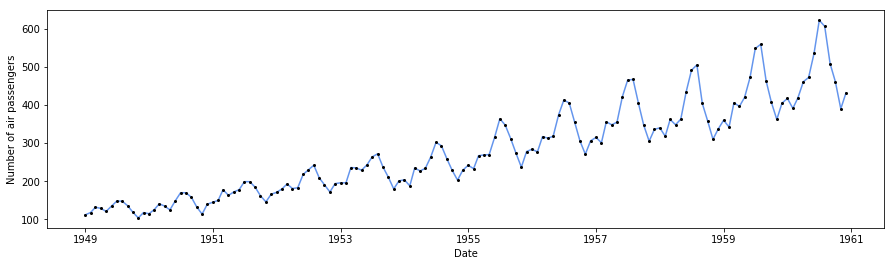
\includegraphics[width=\linewidth]{report/images/airpax_og.png}
    \caption{Original airline passengers data}
    \label{fig:airpax_og}
\end{figure}

The Automatic Statistician report gives a detailed discussion about the additive components it found using the Automatic Bayesian Covariance Discovery (ABCD) algorithm. The components it found are 

\begin{itemize}
    \item a linearly increasing function,
    \item an approximately periodic function with a period of 1.0 years and with approximately linearly increasing amplitude,
    \item a smooth function
    \item uncorrelated noise with linearly increasing standard deviation.
\end{itemize}

It also gives a forecast of an additional year. This forecast can be seen on figure \ref{fig:airpax_as_forecast}, in addition to an extrapolation of the data (before the dashed vertical line). The predicted additional year makes sense to us as a logical continuation of the time series.

\begin{figure}[!ht]
    \centering
    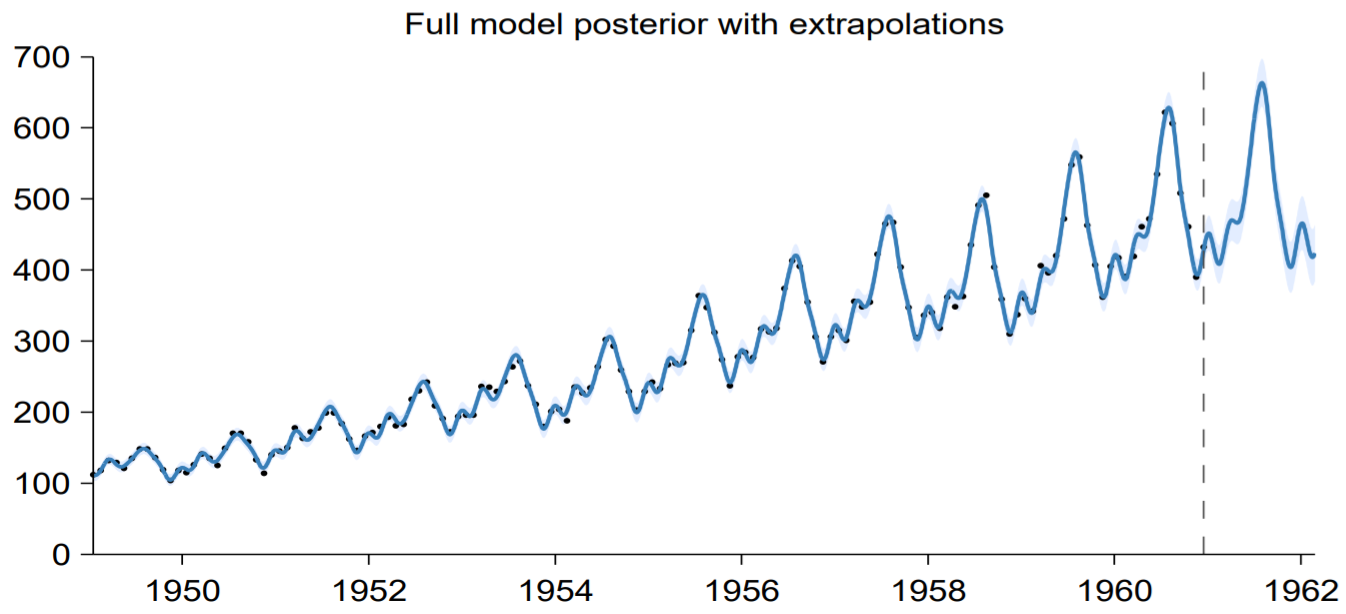
\includegraphics[width=\linewidth]{report/images/airpax_as_forecast.png}
    \caption{Forecast for an additional year by Automatic Statistician}
    \label{fig:airpax_as_forecast}
\end{figure}

We also made a forecast of an additional year by ourselves. We first checked whether or not the time series was stationary, which is a prerequisite to use Autoregressive integrated moving average (ARIMA). The time series is not stationary as the rolling mean is not at all constant, as can be seen on figure \ref{fig:airpax_rolling_mean}. The Augmented Dickey-Fuller (ADF) test confirms this, as the p-value is 0.992.

\begin{figure}[!ht]
    \centering
    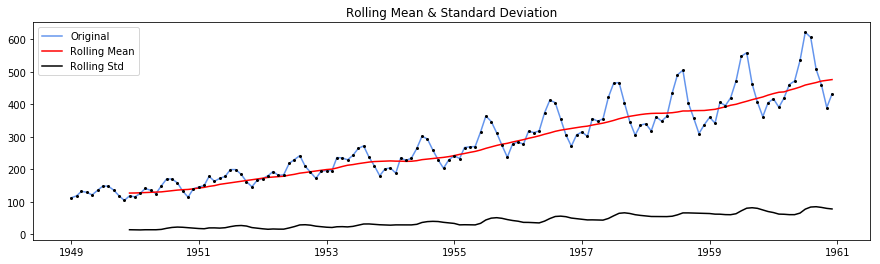
\includegraphics[width=\linewidth]{report/images/airpax_rolling_mean.png}
    \caption{Rolling mean and standard deviation of the time series}
    \label{fig:airpax_rolling_mean}
\end{figure}

As a consequence, we chose to log scale the signal and apply a differencing step to eliminate the non-stationarity. We then decompose this series to have a view on the trend, season and residual component. These different components can be seen on figure \ref{fig:airpax_log_decomp}.

\begin{figure}[!ht]
    \centering
    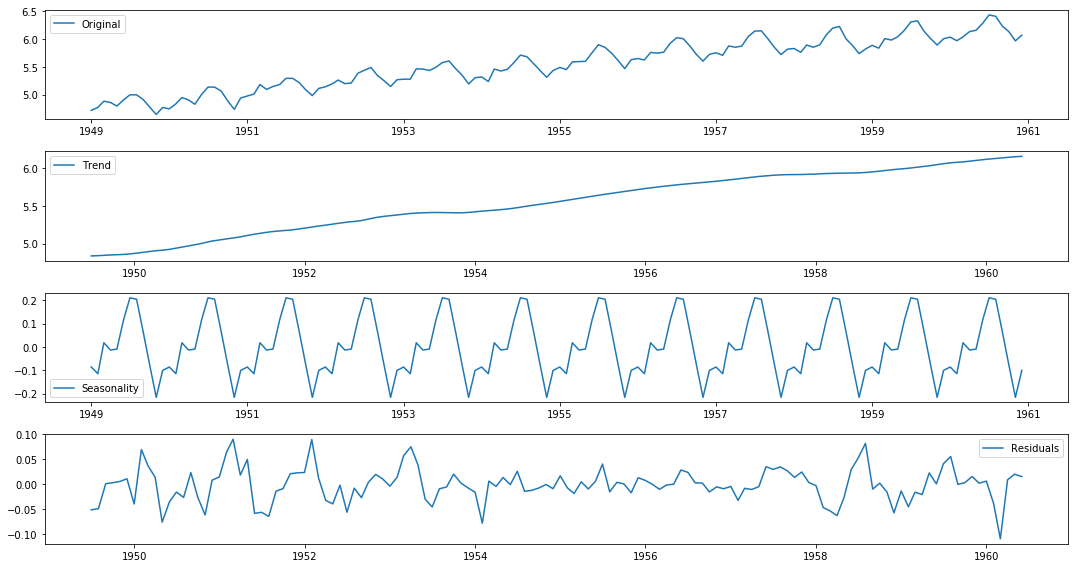
\includegraphics[width=\linewidth]{report/images/airpax_log_decomp.png}
    \caption{Original log-scaled time series, the trend component, the seasonality component and the residuals component}
    \label{fig:airpax_log_decomp}
\end{figure}

Subsequently we can use this scaled series to find the $P$, $D$ and $Q$ parameters for the ARIMA model, we find the values 2,1 and 2 respectively. We show the extrapolation and forecast made by the ARIMA model on the log scaled series in figure \ref{fig:airpax_arima}.

\begin{figure}[!ht]
    \centering
    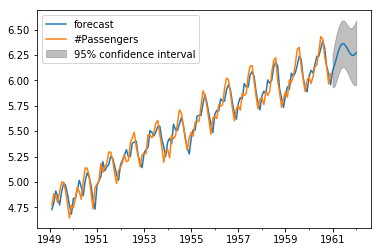
\includegraphics[width=\linewidth]{report/images/airpax_arima.png}
    \caption{Extrapolation and forecast of the ARIMA model}
    \label{fig:airpax_arima}
\end{figure}

Since the forecast of the ARIMA model doesn't seem very accurate, we tried the Seasonal Auto-Regressive Integrated Moving Average with eXogenous regressors (SARIMAX) model. The parameters are picked by performing a brute force search in the range of of 0 to 2 inclusive. At the end of the brute force, the parameters with the best Akaike Information Criterion (AIC) are chosen. The AIC is a measure of how well the model fits the data. The best parameters were (2, 1, 2), (0,2,2) for \textit{(p,d,q) x (P, D, Q)} respectively. The AIC with these parameters is approximately $715.16$. A forecast using the SARIMAX model can be seen on figure \ref{fig:airpax_sarimax} in orange, in combination with the $95\%$-confidence interval in shaded gray.

\begin{figure}[!ht]
    \centering
    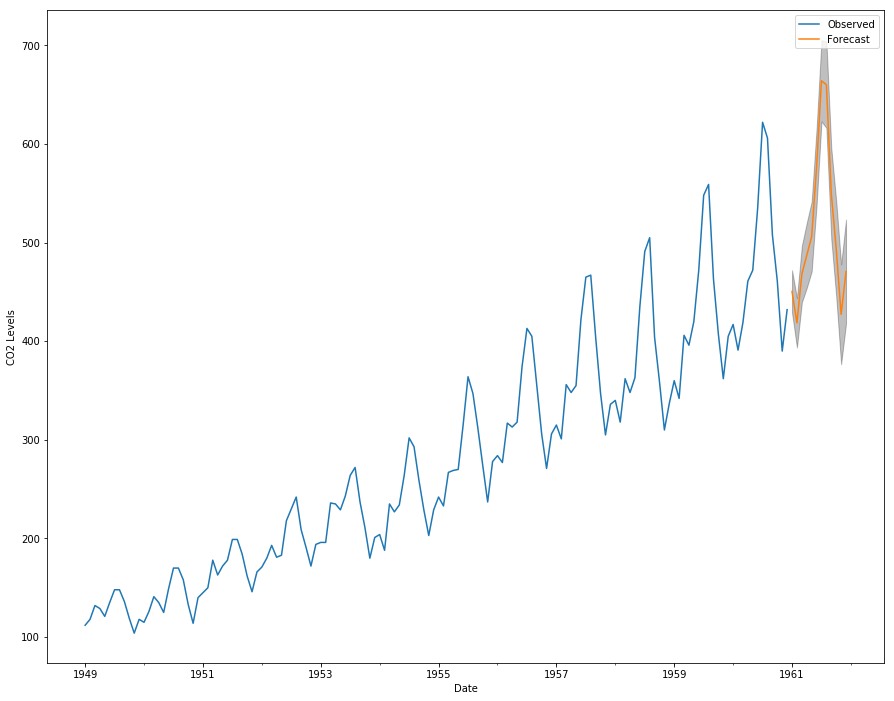
\includegraphics[width=\linewidth]{report/images/airpax_sarimax.png}
    \caption{Forecast using the SARIMAX model}
    \label{fig:airpax_sarimax}
\end{figure}

\section{Conclusion}
\label{sec:conclusion}

From the creative part we can conclude the following things.
The accuracy of the regression analysis of Automatic Statistician is limited to the use of linear models, while this is acceptable for simple datasets such as the affairs dataset, these simple models may not be able to interpret complex datasets correctly. Although the model we found on the website is limited to linear models, research has been done on using ensemble methods as well \cite{moola2015a}. The use of only linear models doesn't only impact the accuracy of predictions, but also the accuracy of revealing relationships between the variables and the target variable. We believe using ensemble models in finding relationships would therefore be a useful improvement to the Automatic Statistician.

The accuracy and the amount of information the Automatic Statistician gives on time series is definitely better than given by its regression part. It took us quite some research to find a way to achieve comparable results to those of the Automatic Statistician in the forecast. The information given about the additive components of the time series are thoroughly explained in the generated report.\\

The Automatic Statistician is a useful tool for people with limited knowledge in statistics. However, due to the fact that the regression part has limited capabilities, it shouldn't be used to accurately describe a regression dataset. Time series can however be accurately interpreted and predicted by the Automatic Statistician. The whole can be definitely be used as a first step towards understanding data, we do believe that it is not yet ready as a standalone tool.

\bibliography{references}
\bibliographystyle{IEEEtran}

\end{document}
